\documentclass{beamer}

\usetheme{metropolis}

\usepackage[ngerman]{babel}
\usepackage[autostyle=true,german=quotes]{csquotes}
\usepackage[linewidth=1pt]{mdframed}
\usepackage{hyperref}
\usepackage{makecell}
\usepackage{pifont}
\usepackage{tikz}
\usetikzlibrary{positioning, calc, arrows, fit, decorations.pathreplacing, shapes, shapes.multipart, snakes}
\usepackage{verbatim}
\usepackage{textcomp}
\usepackage{centernot}
\usepackage{tabularx}
\usepackage{ulem}
%\usepackage{pdfpages}

\batchmode

\hypersetup{
	colorlinks,
	urlcolor=blue,
	linkcolor=black % for ToC
}
\newenvironment{qaa}[1]{
	#1

	\begin{mdframed}
		\small
}{
	\end{mdframed}
}

\newcommand{\true}{\ding{51}}
\newcommand{\false}{\ding{55}}
\newcommand{\code}[1]{
	\begin{mdframed}
		\verbatiminput{#1}
	\end{mdframed}
}


\title{Tutorium 07: Unifikation}
% \subtitle{}
\author{David Kaufmann}
\institute{Tutorium Programmierparadigmen am KIT}
\date{14. Dezember 2022}

\begin{document}

\begin{frame}
	\titlepage
\end{frame}

\section{Unifikation}

\begin{frame}{Welche Probleme löst die Unifikation?}
  \begin{align*}
    \functor{state}{\pa{l}, \pa{l}, \pa{l}, \pa{l}} &\plsunify \functor{state}{M, W, Z, K} \\
    \functor{opposite}{M, M_2}                       &\plsunify \functor{opposite}{\pa{l}, \pa{r}} \\
    Z                                               &\plsunify K \\
  \end{align*}

  \only<1>{
    \begin{itemize}
      \item Unifikation löst Gleichungssysteme von baumförmigen Termen (hier: Prolog-Terme).
      \item Eingabe: Menge $C = \{ \theta_l^1 \plsunify \theta_r^1, ..., \theta_l^n \plsunify \theta_r^n \}$
      \begin{itemize}
        \item Alle $\theta_{\{l, r\}}^i$ sind Bäume und können Variablen enthalten.
      \end{itemize}
      \item Ausgabe: \emph{Unifikator} $\sigma$, sodass $\sigma(\theta_l^i) = \sigma(\theta_r^i)$.
      \begin{itemize}
        \item Wenn $C$ nicht unifizierbar (bspw. $X = \functor{f}{X}$): \texttt{fail}
      \end{itemize}
    \end{itemize}
  }

  \only<2>{
    Mehrere mögliche Lösungen:

    \begin{align*}
      \sigma_1 &=
        \unifier{\su{M_2}{\pa{r}}} \circ
        \unifier{\su{K}{\pa{l}}} \circ
        \unifier{\su{Z}{\pa{l}}} \circ
        \unifier{\su{W}{\pa{l}}} \circ
        \unifier{\su{M}{\pa{l}}} \\
      \sigma_2 &=
        \unifier{\su{M_2}{\pa{r}}} \circ
        \unifier{\su{K}{\pa{l}}} \circ
        \unifier{\su{Z}{\pa{K}}} \circ
        \unifier{\su{W}{\pa{l}}} \circ
        \unifier{\su{M}{\pa{l}}}
    \end{align*}

    \begin{itemize}
      \item I.d.R. suchen wir nach \emph{einem} allgemeinsten Unifikator (mgu).
      \item mgu $\approx$ minimaler Unifikator, der $C$ löst.
    \end{itemize}
  }
\end{frame}

\begin{frame}{Prolog-Unifikation}
  Unifiziert:

  \begin{align*}
    A &\plsunify \pa{x} \\
    B &\plsunify \functor{f}{X} \\
    C &\plsunify \functor{g}{C} \\
    \functor{f}{\pa{x}, D, \pa{z}} &\plsunify \functor{f}{\pa{x}, \pa{y}, E} \\
    \functor{func}{F, \functor{func}{G, \pa{z}}} &\plsunify \functor{func}{\pa{x}, \functor{func}{\pa{y}, F}} \\
    \functor{g}{\pa{x}, H, \pa{z}} &\plsunify \functor{f}{\pa{x}, H, H} \\
    \functor{f}{\functor{g}{\pa{z}}} &\plsunify \functor{f}{J}
  \end{align*}

	Ergebnis: Entweder \textbf{fail} oder ein Unifikator.
\end{frame}

% https://tex.stackexchange.com/questions/57441/how-to-include-existing-pdf-slides-into-my-beamer-presentation
{
\setbeamercolor{background canvas}{bg=}
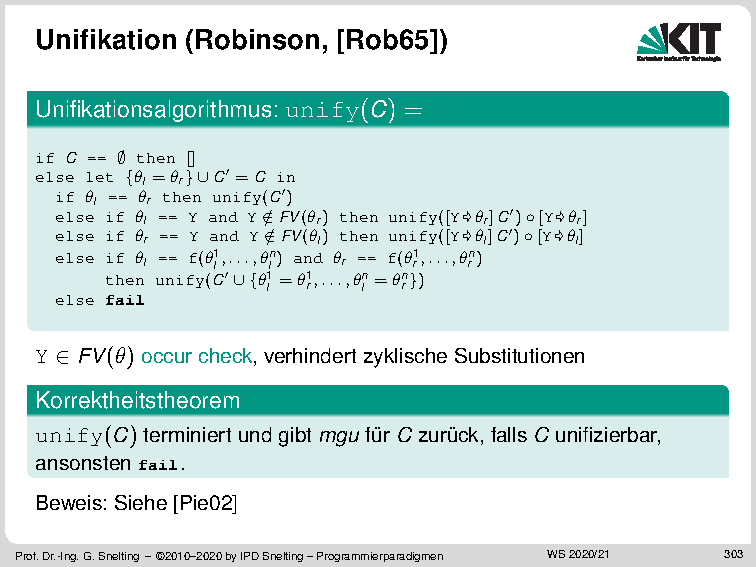
\includepdf{robinson.pdf}
}

\begin{frame}{Robinson-Algorithmus: Zeile für Zeile}
  \only<1>{
    \begin{align*}
      &\texttt{if} \;\; C == \emptyset \;\; \texttt{then} \;\; [] \\
      &\texttt{else let} \;\; \{ \theta_l \plsunify \theta_r \} \cup C' = C \;\; \texttt{in}
    \end{align*}

    \begin{itemize}
      \item Ist das Gleichungssystem $C$ leer, ist es schon gelöst \\
            $\leadsto$ wir brauchen nichts zu ersetzen.
      \item Andernfalls betrachten wir \emph{eine} der Gleichungen: $\theta_l \plsunify \theta_r$.
      \begin{itemize}
        \item \emph{Beliebige Auswahl möglich}.
        \item Die restlichen Gleichungen merken wir uns als $C'$.
      \end{itemize}
    \item Beispiel:\\
          $C = \{ X \plsunify \pa{a}, Y \plsunify \functor{f}{X}, \functor{f}{Z} \plsunify Y \}$\\
          $\theta_l = X, \theta_r = \pa{a}, C' = \{ Y \plsunify \functor{f}{X}, \functor{f}{Z} \plsunify Y \}$
    \end{itemize}
  }

  \only<2>{
    \begin{align*}
      &\texttt{if} \;\; \theta_l == \theta_r \;\; \texttt{then unify}(C')
    \end{align*}

    \begin{itemize}
      \item Wenn die Gleichung trivial ist (auf beiden Seiten steht schon das gleiche), brauchen wir auch nichts zu ersetzen.
      \item Wir müssen also nur $C'$ unifizieren.
      \item Verschiedene Gleichheitsrelationen:
      \begin{itemize}
        \item $A \plsunify B$: Element von $C$, behandeln wir wie eine Datenstruktur.
        \item $A == B$: Vergleichsoperator
        \item $A = B$: Meta-Gleichheitsoperator, Notation für Pattern-Matching
      \end{itemize}
    \end{itemize}
  }

  \only<3>{
    \begin{align*}
      &\texttt{else if} \;\; \theta_l == Y \;\; \texttt{and} \;\; Y \not\in FV(\theta_r) \;\; \\
      &\; \texttt{then unify}(\unifier{\su{Y}{\theta_r}} C') \circ \unifier{\su{Y}{\theta_r}} \\
    \end{align*}

    \begin{itemize}
      \item Steht auf der linken Seite eine Variable, so wird diese ersetzt.
      \begin{itemize}
        \item $\theta_l == Y$: \enquote{Ist der Term $\theta_l$ eine Variable $Y$?}
        \item $Y \not\in FV(\theta_r)$: \emph{occurs check}, $Y$ darf sich nicht selbst einsetzen.
      \end{itemize}
      \item Wir ersetzen in $C'$ dann $Y$ durch $\theta_r$.
      \item Substitution $\unifier{\su{Y}{\theta_r}}$ wird als Ergebnis vorgemerkt.
      \item Beispiel: $\theta_l = X$ \true, $X \not\in FV(\theta_r) = FV(\pa{a}) = \emptyset$ \true, d.h.\\
            Ergebnis: $\texttt{unify}(\{ Y \plsunify \functor{f}{\pa{a}}, \functor{f}{Z} \plsunify Y \}) \circ \unifier{\su{A}{\pa{a}}}$
    \end{itemize}
  }

  \only<4>{
    \begin{align*}
      &\texttt{else if} \;\; \theta_r == Y \;\; \texttt{and} \;\; Y \not\in FV(\theta_l) \;\; \\
      &\; \texttt{then unify}(\unifier{\su{Y}{\theta_l}} C') \circ \unifier{\su{Y}{\theta_l}} \\
    \end{align*}

    \begin{itemize}
      \item Auch wenn rechts eine Variable steht muss sie ersetzt werden.
      \item Beispiel: $\theta_r = Y$ \true, $Y \not\in FV(\theta_l) = FV(\functor{f}{Z}) = \{ Z \}$ \true, d.h.\\
        Ergebnis: $\texttt{unify}(\{ \functor{f}{Z} \plsunify \functor{f}{\pa{a}} \}) \circ \unifier{\su{Y}{f(Z)}}$
    \end{itemize}
  }

  \only<5>{
    \begin{align*}
      &\texttt{else if} \;\; \theta_l == \functor{f}{\theta_l^1, ..., \theta_r^n} \;\; \texttt{and} \;\; \theta_r == \functor{f}{\theta_r^1, ..., \theta_r^n} \\
      &\; \texttt{then unify}(C' \cup \{ \theta_l^1 \plsunify \theta_r^1, ..., \theta_l^n \plsunify \theta_r^n \})
    \end{align*}

    \begin{itemize}
      \item Steht auf beiden Seiten ein Funktor, extrahieren wir paarweise neue Gleichungen und unifizieren diese mitsamt $C'$.
      \begin{itemize}
        \item Namen der Funktoren \emph{müssen identisch sein}! (hier: \texttt{f})
        \item Parameterzahlen der Funktoren \emph{müssen identisch sein}!
        \item Für Atome: $n = 0$, aber schon abgedeckt durch den ersten Fall.
      \end{itemize}
    \item Beispiel: $\theta_l = \functor{f}{Z}, \theta_r = \functor{f}{\pa{a}}$ \true, $C' = \emptyset$\\
          Ergebnis: $\texttt{unify}(\emptyset \cup \{ Z \plsunify \pa{a} \}) = \unifier{\su{Z}{\pa{a}}}$ (links Variable)
    \end{itemize}
  }
\end{frame}

\begin{frame}{Klausuraufgabe SS21 (8 P.)}
    Gegeben sei die einelementige Menge von Gleichungen
    $$C = \{ \functor{f}{X_1,X_1} = \functor{f}{\functor{f}{X_2,X_3},\functor{f}{X_4, \functor{g}{X_4}}}\} $$

    Führen Sie den Unifikationsalgorithmus nach Robinson durch. Geben Sie bei jedem rekursiven Aufruf die erzeugte Substitution sowie die noch zu unifizierende Menge an.
    
    Geben Sie das Endergebnis in Listenform an.
\end{frame}

\section{Typinferenz}

\begin{frame}{Struktur von Lambda-Termen}
  Lambda-Terme bestehen aus
  \begin{itemize}
    \item \textbf<2>{Lambdas} $\lam{p}{b}$
    \item \textbf<3>{Funktionsanwendungen} $\app{x}{y}$
    \item \textbf<4>{Variablen} $x$, \textbf<5>{Konstanten} $\pa{true}, \pa{17}$
  \end{itemize}

  \only<1>{
    \begin{equation*}
      \lam{a}{\lam{f}{\app{f}{(\app{a}{\pa{true}})}}}
    \end{equation*}
  }

  \only<2>{
    \begin{equation*}
      \underbrace{
        \lam{a}{\underbrace{\lam{f}{\app{f}{(\app{a}{\pa{true}})}}}_{\text{Lambda} \atop p = f, b = \app{f}{(\app{a}{\pa{true}})}}}
      }_{
        \text{Lambda} \atop
        p = a, b = \lam{f}{\app{f}{(\app{a}{\pa{true}})}}
      }
    \end{equation*}
  }

  \only<3>{
    \begin{equation*}
      \lam{a}{\lam{f}{\underbrace{\app{f}{
        \underbrace{
         (\app{a}{\pa{true}})
        }_{\text{Anwendung} \atop x = a, y = \pa{true}}
      }}_{\text{Anwendung} \atop x = f, y = \app{a}{\pa{true}}}}}
    \end{equation*}
  }

  \only<4>{
    \begin{equation*}
      \lam{a}{\lam{f}{\app{
        \underbrace{f}_{\text{Variable}}
      }{(\app{
        \underbrace{a}_{\text{Variable}}
      }{\pa{true}})}}}
    \end{equation*}
  }

  \only<5>{
    \begin{equation*}
      \lam{a}{\lam{f}{\app{f}{(\app{a}{\underbrace{\pa{true}}_{\text{Konstante}}})}}}
    \end{equation*}
  }
\end{frame}

\begin{frame}{Lambda-Terme als Bäume}
  Wir können Lambda-Terme also als Bäume mit Lambda- und Anwendungsknoten und Variablen- und Konstantenblättern betrachten, um ihre Struktur zu untersuchen:

  \begin{columns}
    \begin{column}{0.5\textwidth}
      \begin{figure}
      \begin{tikzpicture}
        \node {$\lambda a$}
          [level distance=10mm]
          child {node {$\lambda f$}
            child {node {@}
              child {node {$f$}}
              child {node {@}
                child {node {$a$}}
                child {node {$\pa{true}$}}
              }
            }
          }
        ;
      \end{tikzpicture}
      \end{figure}
    \end{column}
    \begin{column}{0.35\textwidth}
      \begin{equation*}
        \lam{a}{\lam{f}{\app{f}{(\app{a}{\pa{true}})}}}
      \end{equation*}
    \end{column}
  \end{columns}
\end{frame}

\begin{frame}{Cheatsheet: Typisierter Lambda-Kalkül}
  \begin{mathpar}
    \inferrule{
      \Gamma{}(t) = \tau
    }{
      \Gamma \vdash t : \tau
    } \textrm{\textsc{Var}}
    \and
    \inferrule{
      \Gamma \vdash f : \phi \to \alpha \\
      \Gamma \vdash x : \phi
    }{
      \Gamma \vdash \app{f}{x} : \alpha
    } \textrm{\textsc{App}}
    \and
    \inferrule{
      \Gamma{}, p : \pi \vdash b : \rho
    }{
      \Gamma \vdash \lam{p}{b} : \pi \to \rho
    } \textrm{\textsc{Abs}}
  \end{mathpar}

  \begin{itemize}
    \item Typvariablen: $\tau$, $\alpha$, $\pi$, $\rho$
    \item Funktionstypen: $\tau_1 \to \tau_2$, rechtsassoziativ
    \item (Weitere Typen: Listen, Tupel, etc.)
    \item \emph{Typisierungsregeln sind eindeutig}: Eine Regel pro Termform
  \end{itemize}
\end{frame}

\begin{frame}{(Allgemeine) Typisierungsregel für Variablen}
	\begin{itemize}
		\item \tikz[baseline, remember picture]{\node [fill=green!20,draw] (varRetL) {\enquote{Der Typkontext $\Gamma$ enthält einen Typ $\tau$ für $t$.}};}
	\end{itemize}

	\begin{mathpar}
		\inferrule{
			\tikz[baseline, remember picture]{\node[fill=green!20,draw] (varRet) {$\Gamma{}(t) = \tau$};}
		}{
			\tikz[baseline, remember picture]{\node[fill=blue!20,draw] (varShow) {
				$\Gamma \vdash t : \tau$
			};}
		} \textrm{\textsc{Var}}
	\end{mathpar}

	\begin{itemize}
		\item Daraus folgt:
		\item \tikz[baseline, remember picture]{\node [fill=blue!20,draw] (varShowL) {\enquote{Variable $t$ hat im Kontext $\Gamma$ den Typ $\tau$.}};}
	\end{itemize}

	\tikz[overlay, remember picture]{
		\draw[->] (varShowL) edge [bend left] (varShow);
		\draw[->] (varRetL) edge [bend right] (varRet);
	}
\end{frame}

\newcommand{\tikzmark}[3]{\tikz[baseline, remember picture]{
	\node[fill=#1,draw] (#2) {#3};
}}

\begin{frame}{Typisierungsregel für Funktionsanwendungen}
	\begin{itemize}
		\item \tikzmark{green!20}{fTypeL}{\enquote{$f$ ist im Kontext $\Gamma$ eine Funktion, die $\phi$s auf $\alpha$s abbildet.}}
		\item \tikzmark{red!20}{aTypeL}{\enquote{$x$ ist im Kontext $\Gamma$ ein Term des Typs $\phi$.}}
	\end{itemize}
	\begin{mathpar}
		\inferrule{
			\tikzmark{green!20}{fType}{$\Gamma \vdash f : \phi \to \alpha$} \\
			\tikzmark{red!20}{aType}{$\Gamma \vdash x : \phi$}
		}{
			\tikzmark{blue!20}{eType}{$\Gamma \vdash \app{f}{x} : \alpha$}
                } \textrm{\textsc{App}}
	\end{mathpar}

	\begin{itemize}
		\item Daraus folgt:
		\item \tikzmark{blue!20}{eTypeL}{\enquote{$x$ eingesetzt in $f$ ergibt einen Term des Typs $\alpha$.}}
	\end{itemize}

	\tikz[overlay, remember picture]{
		\draw[->] (fTypeL) edge [bend right] (fType);
		\draw[->] (aTypeL) edge [bend left] (aType);
		\draw[->] (eTypeL) edge [bend left] (eType);
	}
\end{frame}

\begin{frame}{Typisierungsregel für Lambdas}
	\begin{itemize}
		\item \tikzmark{green!20}{contextL}{\enquote{Unter Einfügung des Typs $\pi$ von $p$ in den Kontext...}}
		\item \tikzmark{red!20}{bodyTypeL}{\enquote{... ist $b$ als Funktion von $p$ typisierbar.}}
	\end{itemize}

	\begin{mathpar}
		\inferrule{
			\tikzmark{green!20}{context}{$\Gamma{}, p : \pi$} \\
			\tikzmark{red!20}{bodyType}{$\vdash b : \rho$}
		}{
			\tikzmark{blue!20}{absType}{$\Gamma \vdash \lam{p}{b} : \pi \to \rho$}
                } \textrm{\textsc{Abs}}
	\end{mathpar}

	\begin{itemize}
		\item Daraus folgt:
		\item \tikzmark{blue!20}{absTypeL}{\enquote{$\lam{p}{b}$ ist eine Funktion, die $\pi$s auf $\rho$s abbildet}}
	\end{itemize}

	\tikz[overlay, remember picture]{
		\draw[->] (bodyTypeL) edge [bend left] (bodyType);
		\draw[->] (contextL) edge [bend right] (context);
		\draw[->] (absTypeL) edge [bend left] (absType);
	}
\end{frame}

\begin{frame}{Typinferenz}
	Vorgehensweise zur Typinferenz:
	\begin{itemize}
		\item Stelle Typherleitungsbaum auf
		\begin{itemize}
			\item In jedem Schritt werden neue Typvariablen $\alpha_i$ angelegt
			\item Statt die Typen direkt im Baum einzutragen, werden Gleichungen in einem Constraint-System eingetragen
		\end{itemize}
		\item Unifiziere Constraint-System zu einem Unifikator
		\begin{itemize}
			\item Robinson-Algorithmus, im Grunde wie bei Prolog
                        \item I.d.R.: Allgemeinster Unifikator (findet man per Robinson)
		\end{itemize}
	\end{itemize}
\end{frame}

{
\setbeamercolor{background canvas}{bg=}
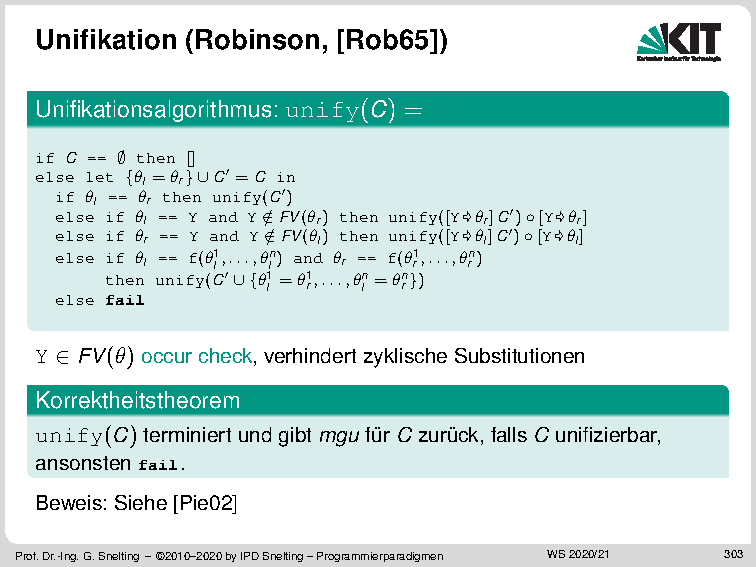
\includepdf{robinson.pdf}
}

{
\setbeamercolor{background canvas}{bg=}
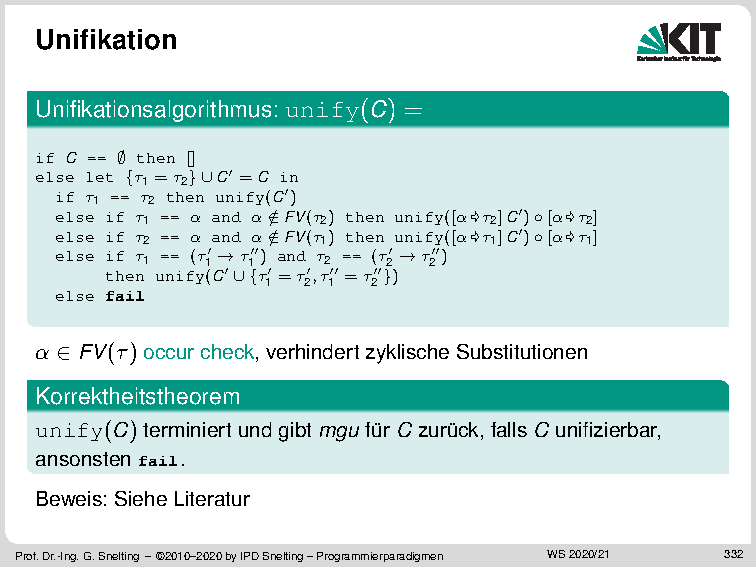
\includepdf{robinson2.pdf}
}

\begin{frame}{Unifikation für Typinferenz}
  \emph{Typen kann man auch als Funktoren darstellen}:

  \begin{align*}
    \tau_1 \to \tau_2   && \equiv && \texttt{func}(\tau_1, \tau_2) \\
    \left[ \tau \right] && \equiv && \texttt{list}(\tau) \\
                        && \text{etc.}
  \end{align*}
\end{frame}

\begin{frame}{Typinferenz: Übungsaufgaben}
	\only<1>{
	\begin{mathpar}
		\inferrule{
			...
		}{
                  f : \textrm{int} \to \beta \vdash \lam{x}{\app{f}{x}} : \alpha_1
                } \textrm{\textsc{Abs}}
	\end{mathpar}

	\begin{itemize}
		\item \enquote{Finde den allgemeinsten Typen $\alpha_1$ von $\lam{x}{\app{f}{x}}$}
	\end{itemize}
	}

	\only<2>{
	\begin{mathpar}
		\inferrule{
			...
		}{
                  \vdash \lam{f}{\lam{x}{\app{(\app{f}{x})}{x}}} : \alpha_1
                } \textrm{\textsc{Abs}}
	\end{mathpar}

	\begin{itemize}
          \item \enquote{Finde den allgemeinsten Typen $\alpha_1$ von $\lam{f}{\lam{x}{\app{(\app{f}{x})}{x}}}$}
	\end{itemize}
	}


	Erinnerung:

	\begin{itemize}
		\item Baum mit durchnummerierten $\alpha_i$ aufstellen
		\item Constraints sammeln:
	\end{itemize}

	\begin{columns}
		\scriptsize
		\begin{column}{0.3\textwidth}
                  \begin{mathpar}
    \inferrule{
      \Gamma{}(t) = \alpha_j
    }{
      \Gamma \vdash t : \alpha_i
    } \textrm{\textsc{Var}}
                  \end{mathpar}

                  \center
                        Constraint:\\$\{ \alpha_i = \alpha_j \}$
		\end{column}
		\begin{column}{0.3\textwidth}
                  \begin{mathpar}
    \inferrule{
      \Gamma \vdash f : \alpha_j \\
      \Gamma \vdash x : \alpha_k
    }{
      \Gamma \vdash \app{f}{x} : \alpha_i
    } \textrm{\textsc{App}}
                  \end{mathpar}
\center
			Constraint:\\$\{ \alpha_j = \alpha_k \to \alpha_i \}$
		\end{column}
		\begin{column}{0.3\textwidth}
                  \begin{mathpar}
    \inferrule{
      \Gamma{}, p : \alpha_j \vdash b : \alpha_k
    }{
      \Gamma \vdash \lam{p}{b} : \alpha_i
    } \textrm{\textsc{Abs}}
                  \end{mathpar}
                        \center
			Constraint:\\$\{ \alpha_i = \alpha_j \to \alpha_k \}$
		\end{column}
	\end{columns}

	\begin{itemize}
		\item Constraint-System auflösen
	\end{itemize}
\end{frame}

\begin{frame}{Nächste Woche (21. Dezember 2022)}
    \begin{itemize}
        \item Mehr...
        \begin{itemize}
            \item ...Prolog?
            \item ...Unifikation?
            \item ...Typherleitung?
            \item ...Haskell?
        \end{itemize}
    \end{itemize}
\end{frame}

\end{document}
